\documentclass[11pt,class=report,crop=false]{standalone}
\usepackage{exo7hilisit}

\begin{document}


\entete{Hilisit}{Capacité mathématiques}

\titre{\'Equations différentielles -- Partie 4 : $\boldsymbol{y'=ay+b}$ et $\boldsymbol{y'=ay+f}$} 

\bigskip
\bigskip


%%%%%%%%%%%%%%%%%%%%%%%%%%%%%%%%%%%%%%%%%%%%%%%%%%%%%%%%%%%%
%\section{$y'=ay+b$ et $y'=ay+f$}

\exercice{}
\enonce
Pour chacune des équations différentielles $(E)$ suivantes, 
 \begin{itemize}
  \item déterminer l'équation homogène associée,
  \item trouver les solutions $y_h(x)$ de cette équation homogène,
  \item vérifier que la fonction $y_p(x)$ est bien solution de l'équation différentielle $(E)$,
  \item en déduire toutes les solutions de $(E)$.
\end{itemize} 
 
 \begin{enumerate}
  \item $y'=-y+x^2+1$, $y_p(x)=x^2-2x+3$
  \item $y'=y+2\cos(x)$, $y_p(x)=\sin(x)-\cos(x)$ 
  \item $y'=3y+xe^{2x}$, $y_p(x)=-(x+1)e^{2x}$
\end{enumerate} 
\finenonce

\finexercice

\exercice{}
\enonce
Pour chacune des équations différentielles $(E)$ suivantes, 
 \begin{itemize}
  \item déterminer l'équation homogène associée,
  \item trouver les solutions $y_h(x)$ de cette équation homogène,
  \item trouver une solution particulière $y_p(x)$ en vous aidant des indications,
  \item en déduire toutes les solutions de $(E)$.
\end{itemize} 
 
 \begin{enumerate}
  \item $y'+2y=5$, chercher une solution particulière sous la forme d'une fonction constante.  % 5
  \item $2y'-3y=e^{-x}$, chercher une solution particulière sous la forme $ke^{-x}$ où $k$ est une constante à déterminer. % -1/5e^{-x}$
  \item $y'=y + x^2$, chercher une solution particulière sous la forme $ax^2+bx+c$.    % - x^2 - 2 x - 2
\end{enumerate} 
\finenonce

\finexercice




\exercice{}
\enonce

Le dessin représente quelques solutions de l'équation différentielle $(E) : y'=2y+x^2e^x$.

\begin{center}
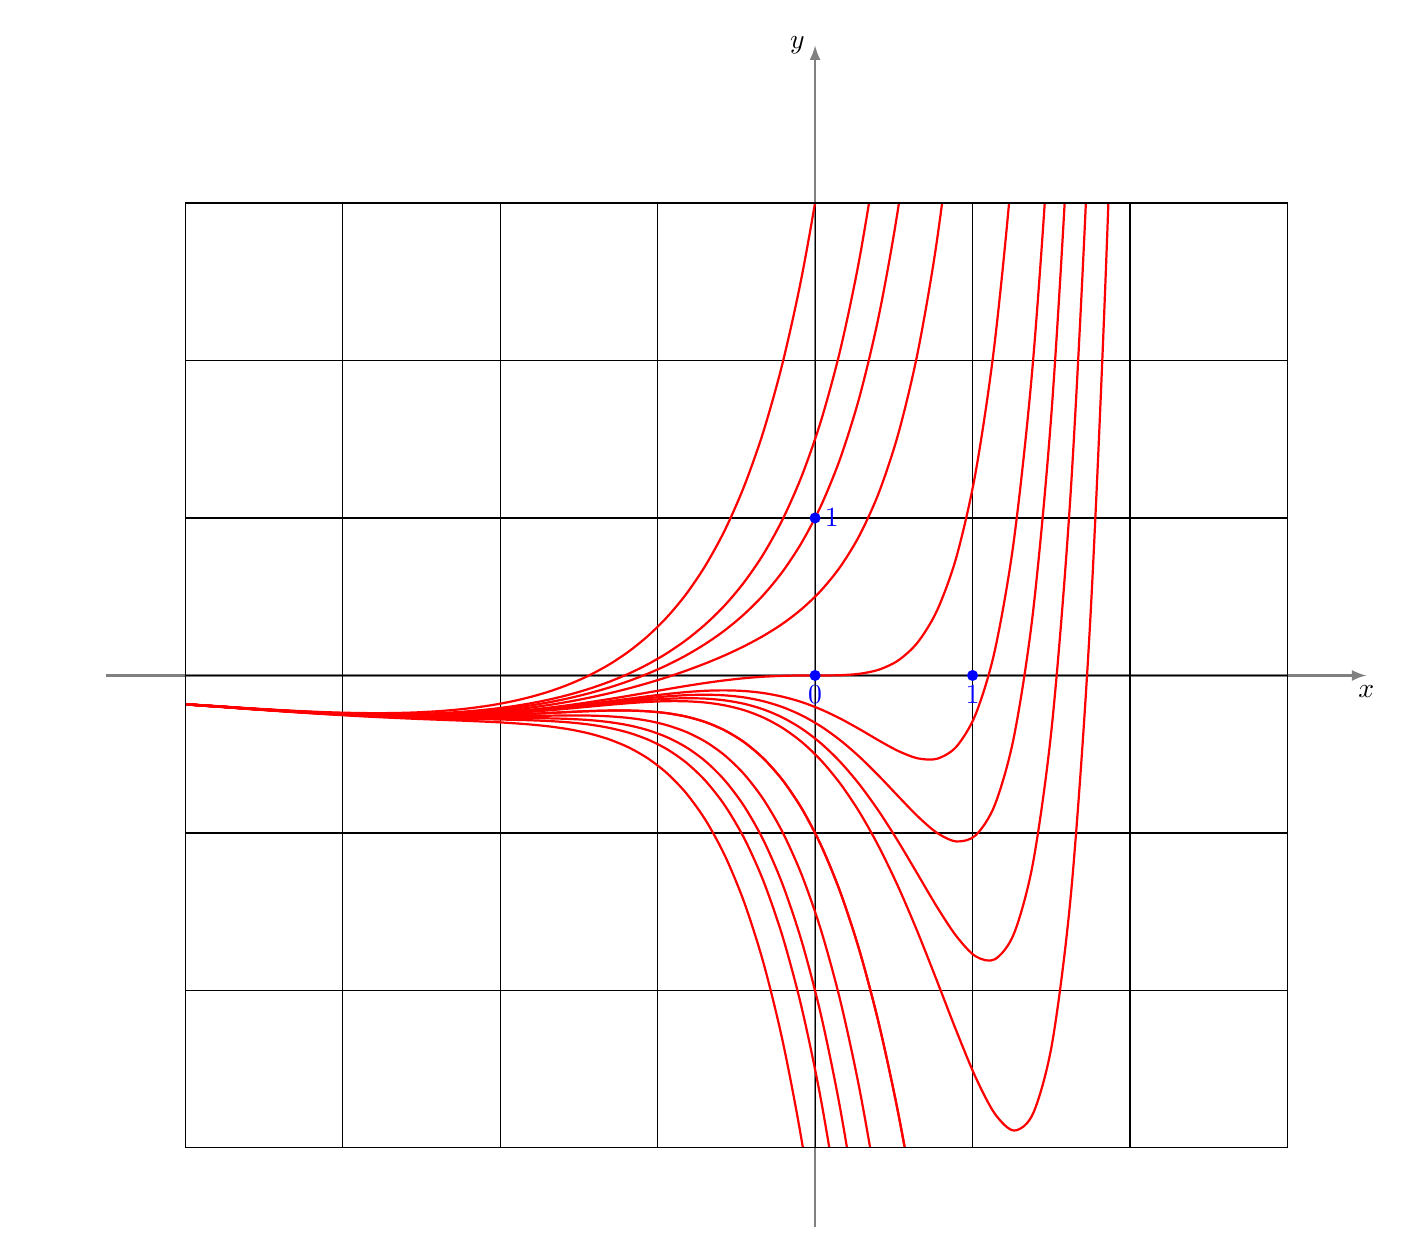
\begin{tikzpicture}[scale=2]

  \draw[->,>=latex,thick,gray] (-4.5,0) -- (3.5,0) node[below,black] {$x$};
  \draw[->,>=latex,thick,gray] (0,-3.5) -- (0,4) node[left,black] {$y$};
  \draw (-4,-3) grid (3,3);
\begin{scope}
    \clip (-5,-3) rectangle (3,3);


\foreach \k in {-1.5,-0.5,0,1,0.5,1,1.5,1.6,1.7,1.8,2,2.5,3,3.5,5} {
  \draw[thick, color=red,domain=-4:2, smooth, samples=50] plot (\x,{\k*exp(2*\x)-((\x)^2+2*\x+2)*exp(\x)}); 
}

\end{scope}

\fill[blue] (0,0)  circle (1pt) node [below] {$0$}; 
\fill[blue] (1,0)  circle (1pt) node [below] {$1$}; 
\fill[blue] (0,1)  circle (1pt) node [right] {$1$};

\draw (-4,-3) rectangle (3,3);

\end{tikzpicture}
\end{center}


\begin{enumerate}
  \item Tracer la tangente à la courbe solution qui passe par le point $(0,0)$. Retrouver son équation par le calcul  grâce à l'équation différentielle.

  \item Tracer la tangente à la courbe solution qui passe par le point $(0,1)$. Retrouver son équation par le calcul grâce à l'équation différentielle.

  \item Tracer la tangente à la courbe solution qui passe par le point $(1,-1)$. Retrouver son équation par le calcul grâce à l'équation différentielle.

  \item Déterminer les solutions $y_h(x)$ de l'équation homogène.

  \item Déterminer une solution particulière $y_p(x)$ sous la forme $(ax^2+bx+c)e^x$.

  \item En déduire toutes les solutions de $(E)$.

\end{enumerate} 
\finenonce

\finexercice



\end{document}
